\chapter{Discussions}

% ------------------------------------------------------------------------------ %
\section{Problèmes rencontrés}
% ------------------------------------------------------------------------------ %

Cette section offre une discussion autour des difficultés qui ont été rencontrées au cours de ce projet. La plupart ont pu être résolues, mais certaines d'entre elles restent encore aujourd'hui sans correctif, en raison d'un manque de temps ou du fait que l'erreur n'émane pas de l'utilisateur, mais plutôt de l'implémentation réalisée par une autre entité (bibliothèque fournie, limites d'un framework choisi, etc.). 

% ------------------------------------------------------------------------------ %
\subsection{Réalisation matérielle de la DevBox}
% ------------------------------------------------------------------------------ %

Lors de la conception de la DevBox, certaines erreurs ont été commises mais elles ont toutes pu être corrigées sur la carte de démonstration. La \cref{sec_hardware_errors} explique toutes les erreurs commises, ainsi que les améliorations qui pourraient être apportées pour une nouvelle version de la carte. \\

Il existe un phénomène actuellement inexplicable se produisant avec les données de la température provenant du BME680 et exposé sur la \cref{fig-bme680_temperature_bug}. Toutes les 12 heures environ, le capteur transmet un \textit{glitch} qui a pour effet de fausser la mesure de température d'un delta de 1.5\,°C. Cet effet est également visible sur la mesure de l'humidité mais avec un impact moindre ($\pm$ 4\,\%). La valeur de la température affichée sur la \cref{fig-bme680_temperature_bug} est calculée à l'aide de la bibliothèque BSEC. Des tests avec les données brutes du BME680 ont toutefois aussi prouver que ce n'est pas la bibliothèque qui altère les données. Malheureusement, le temps a manqué pour explorer ce phénomène plus en détail.

\begin{figure}[ht!]
    \centering
    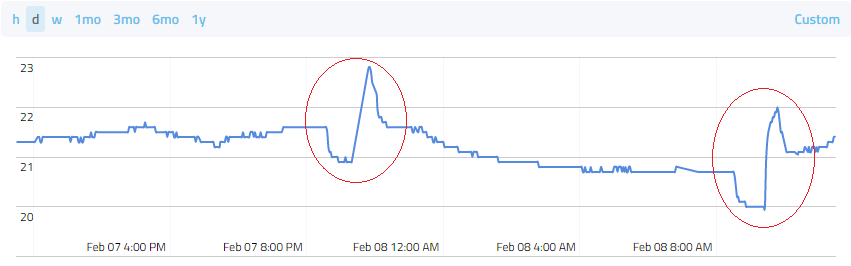
\includegraphics[width=0.7\textwidth]{Figures/bme680_temperature_bug.png}
    \caption{Mesure de la température faussée sur le BME680}
    \label{fig-bme680_temperature_bug}
\end{figure}

% ------------------------------------------------------------------------------ %
\subsection{Développement logiciel de la DevBox}
% ------------------------------------------------------------------------------ %

La programmation du KW41Z a été l'étape qui a demandé le plus d'investissement en terme de temps. La programmation d'un RTOS est complexe et surtout le débogage peut vite devenir difficile en fonction de l'erreur commise. \\

La liste qui suit n'est pas dans un ordre chronologique, mais elle contient les plus principaux problèmes rencontrés : 
\begin{enumerate}
    \item Le débogueur fournit par la FDRM-KW41Z carte d'évaluation n'a pas pu être utilisé pour programmer la DevBox à cause d'un manque de documentation concernant les \textit{jumpers} pour utiliser la carte de développement. Heureusement, un JTAG Link de Segger était compatible avec le KW41Z et a donc été utilisé tout au long du projet pour la programmation et le débogage.
    
    \item Les principaux problèmes liés à la programmation du RTOS proviennent du manque de documentation disponible. En effet, depuis le rachat de Freescale par NXP, certains documents ne sont pas disponibles sous la rubrique documentation du microcontrôleur KW41Z. Il s'agit principalement des documentations se référant à l’OS Abstraction layer de Freescale. La documentation du SDK n'est pas encore intégralement complète sur le site de NXP. Freescale propose cette documentation au format PDF, mais NXP a décidé de la rendre disponible sous forme de page web (\url{http://mcuxpresso.nxp.com/api_doc/dev/224/}), mais plusieurs chapitres ne sont pas disponibles, contrairement au PDF nommé \texttt{Kinetis SDK v.2.0 API Reference Manual}\footnote{\url{https://www.nxp.com/docs/en/reference-manual/KSDK20APIRM.pdf}}. Ce dernier a donc été utilisé comme principale source d'informations.
    
    
    \item Une nouvelle version du SDK est disponible, intitulé KSDK 2.3 ou MCUXpresso SDK selon les plateformes. Suite à cela, NXP a mis à jour son site web, mais malheureusement certains outils ne sont plus fonctionnels. Par exemple, l'outil nommé \texttt{PIN TOOLS}, ayant pour but de faciliter la configuration des pins du microcontrôleur selon de leurs fonctionnalités assignées, n'est maintenant plus accessible pour le KW41Z. Une nouvelle version de l'IDE MCUXpresso est également disponible pour le KW41Z, mais les exemples de l'ancien SDK ne sont pas compatibles avec la nouvelle version. Deux messages\footnote{\url{https://community.nxp.com/thread/466353} \url{https://community.nxp.com/thread/464380}} ont été postés sur le forum d'aide de NXP, dans le but d'obtenir des informations sur le sujet. Ils ont répondu qu'ils étaient conscients des problèmes, mais qu'à l'heure actuelle, le changement de SDK et d'IDE n'est pas envisageable pour le KW41Z.
    
    \item Il y a un problème avec le scanner Bluetooth sur le KW41Z: lorsque l'utilisateur souhaite scanner en permanence les périphériques l'entourant, le scan arrête de transmettre des informations après un laps de temps indéterminé. Cette erreur semble être présente sur le KW41Z depuis septembre 2017, à en croire les divers messages\footnote{\url{https://community.nxp.com/thread/453829}} qui peuvent être lus sur le forum NXP. Pour corriger ce problème, le support de NXP conseille le redémarrage du contrôleur Bluetooth, sans garantir que cela puisse corriger le problème. Il faut ainsi attendre une mise à jour du SDK afin de pouvoir avoir un correctif fonctionnel.
\end{enumerate}

En somme, la documentation éparse de ce microcontrôleur, plus particulièrement au niveau logiciel fait qu'il est souvent plus facile de consulter le code source (si disponible) que de chercher la documentation complète. Le rachat de Freescale par NXP est l'une des causes due à la fusion de certains éléments logiciels entre les deux entités. Cela semble toutefois s'améliorer au fur et à mesure de la publication de nouvelles versions. Le code est très bien structuré et aisément compréhensible, on s'habitue donc assez vite à cette approche. \\

Le support en ligne de NXP a été utilisé à plusieurs reprises. C'est un support très réactif et expérimenté, chaque message posté ayant obtenu une réponse en moins de 24 heures. 


% ------------------------------------------------------------------------------ %
\subsection{Serveur}
% ------------------------------------------------------------------------------ %

L'implémentation du serveur a été grandement facilitée par l'utilisation du langage Python et de ses bibliothèques très complètes. Les seuls problèmes rencontrés sont dus à l'implémentation de l'authentification basée sur les JWT. Après avoir testé différentes bibliothèques, les limitations des premiers tests ont disparu. 

\subsection{Application Android}


La plus grande difficulté de l'application Android provient de l'utilisation du Bluetooth. Même avec l'utilisation de la bibliothèque SweetBlue, il y a tout de même certaines instabilités qui demeurent. Android a pour but d'offrir une couche d'abstraction entre les différents appareils, mais en ce qui concerne le Bluetooth, le comportement diffère encore beaucoup d'un dispositif à un autre. Par exemple, sur une tablette Nexus 9 avec Android 8.0, parfois le pop-up du \textit{passkey} BLE n'est pas affiché. Il est alors nécessaire d'aller dans le menu de notifications afin d'avoir une carte demandant à l'utilisateur de s'appairer. Ce type d'erreur ne se produit pas avec un Samsung Galaxy S7 sous Android 7.0.

% ------------------------------------------------------------------------------ %
\subsection{Démonstrateur}
% ------------------------------------------------------------------------------ %


Pour le démonstrateur, en collaboration avec la DGSI, il a été décidé de tester la connexion de la DevBox sur l'infrastructure SmartCanton. En novembre 2017, un premier test d'intégration a eu lieu entre la DevBox et le réseau LoRaWAN avec la fédération SmartCanton et Orbiwise qui s'est déroulé correctement. La carte a pu rejoindre le réseau et envoyer des données. Orbiwise a gracieusement fourni un compte de test  qui a permis l'utilisation du \textit{Join Server} implémenté par le SmartCanton pour rejoindre le réseau. Cependant, le POC a dû être modifié entre temps et cet accès n'était plus valide. Fin décembre 2017, nous avons voulu retenter l'intégration, mais une erreur au niveau de l'intégration avec Orbiwise a rendu le système non fonctionnel. En raison des fêtes de fin d'année, cette erreur ne pouvait pas être résolues avant les premières semaines de janvier. Nous avons donc décidé de se passer du SmartCanton et de n'utiliser ni la plateforme avec FIWARE pour la partie applicative, ni utiliser le réseau avec le Join Server du SmartCanton. Une démonstration avec The Things Network et Cayenne a été mise en place afin d'avoir un démonstrateur visuel et, surtout, de pouvoir tester les messages LoRaWAN en \textit{uplink} et \textit{downlink}.\\


Pour le démonstrateur final, la plateforme Cayenne a été utilisée pour réaliser un \textit{dashboard}. Néanmoins, la plateforme Cayenne n'est pas encore stable. Voici les quelques erreurs qu'y on été rencontrées et la manière dont celles-ci ont été corrigées : 

\begin{enumerate}
    \item Impossible d'ajouter un périphérique supprimé précédemment: si on supprime un périphérique de son \textit{dashboard}, il est censé réapparaitre lorsqu'une nouvelle trame de données est reçue par Cayenne. Néanmoins, ce périphérique n'est parfois pas recréé. La seule solution est de recommencer à zéro depuis The Things Network, c'est-à-dire supprimer l'application ainsi que les périphériques LoRa.
    
    \item Messages \textit{downlink} non confirmés: selon le guide d'utilisation de Cayenne, les messages \textit{downlink} (de l'application vers le périphérique) génèrent une confirmation visuelle pour l'utilisation. Par exemple, si l'utilisateur appuie sur un bouton pour allumer une LED, celui-ci doit afficher un petit cercle de chargement en attendant la réponse du périphérique. Cependant l'implémentation actuelle de Cayenne ne supporte pas cet état d'attente. La LED apparait tout de suite allumée lorsque l'on appuie sur le bouton, alors qu'aucun message \textit{uplink} n'a été reçu du périphérique. Il n'y a pas de solution à ce problème; il faut attendre une mise à jour de Cayenne. 
    
    \item Capteurs non actualisés sur la plateforme: il arrive parfois que certains capteurs ne soient plus actualisés ou qu'un deuxième capteur, avec le même identifiant et les mêmes données, apparaisse dans le \textit{device}. La première solution est de supprimer le capteur et d'attendre que le \textit{device} envoie quelques nouvelles trames de données (le nombre de trames pour actualiser le \textit{device} est aléatoire, mais il varie entre 1 et 5 trames). Si celui-ci ne réapparait pas, la seule solution est de supprimer entièrement le périphérique. 
    
    \item Plateforme hors ligne: de temps en temps les paquets reçus par The Things Network ne sont pas mis à jour par Cayenne. Le problème provient de leur infrastructure qui passe en maintenance. Malheureusement, aucune communication sur ces maintenances n'est effectuée, le seul moyen étant de visiter le forum et de demander l'état du système. 
\end{enumerate}

Il faut être conscient que les périphériques LoRa sur Cayenne sont encore en \textit{bêta}, raison pour laquelle que le nombre de problèmes est élevé. Pour un service gratuit se trouvant en Bêta, il s'agit d'un très bon portail pour réaliser des tests.

% ------------------------------------------------------------------------------ %
\section{Améliorations possibles}
\label{sec-discuss_enhancements}
% ------------------------------------------------------------------------------ %

Dans l'ensemble, les objectifs initiaux ont pu être réalisés dans ce projet, malgré le fait qu'il reste toutefois des améliorations possibles dans plusieurs domaines. Le rôle de cette section est d'explorer certaines de ces améliorations qui pourraient être implémentées dans une future version du projet.

% ------------------------------------------------------------------------------ %
\subsection{Sécurité}
% ------------------------------------------------------------------------------ %

La sécurité a certes été explorée dans le cadre de ce projet, mais celle-ci peut encore être améliorée. Voici dans les quelques sections qui suivent les principaux axes à explorer.

\subsubsection{Stockage des clés}

À l'heure actuelle, l'AppKey est stockée dans le KW41Z (cf. \cref{fig-diagram_keys_devbox}). Ce n'est pas idéal pour un projet commercial, car cela implique que l'AppKey soit transférée à chaque initialisation. Celle-ci doit plutôt être stockée à l'intérieur du module LoRaWAN puisqu'il dispose d'un coffre fort nommé STSAFE (cf. \cref{sec-hardware_lora_module} et \cref{sec-mcu_stsafe}) prévu à cet effet. Comme évoqué en \cref{sec-mcu_stsafe}, la documentation de ce module n'est à l'heure actuelle pas publique; comme pour beaucoup de circuits de cryptographie, il faut accepter des conditions spéciales envers le fabricant afin d'avoir accès aux guides d'utilisation et aux spécifications de ce module. Cela reste néanmoins l'une des meilleures solutions pour garder en lieu sûr les clés sur un système embarqué.
La situation actuelle n'est que temporaire et doit être résolue en utilisant un stockage unique à l'intérieur du CMWX1ZZABZ, comme illustré sur la \cref{fig-diagram_keys_devbox}.

\begin{figure}[ht!]
    \centering
    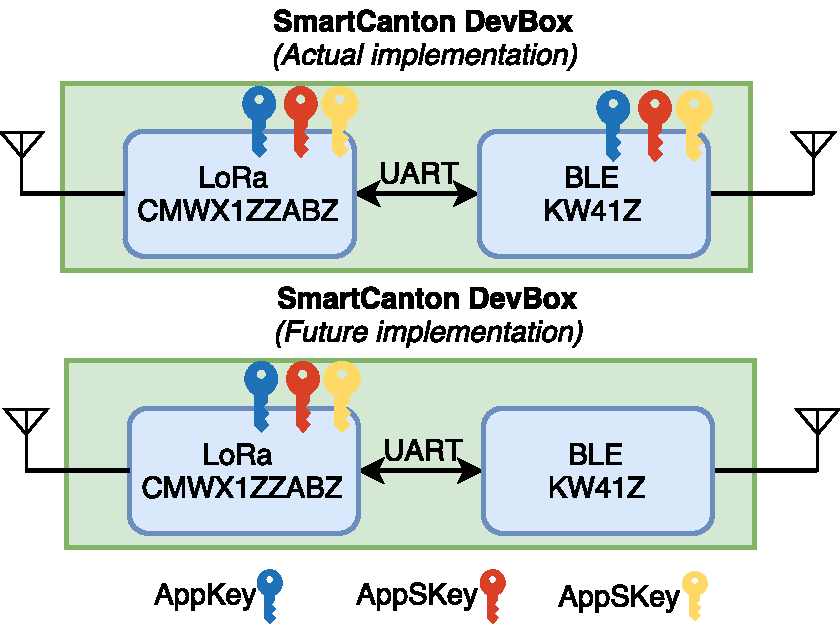
\includegraphics[width=0.6\textwidth]{Figures/diagram_keys_devbox.pdf}
    \caption{Amélioration du stockage des clés sur le KW41Z}
    \label{fig-diagram_keys_devbox}
\end{figure}


\subsubsection{Confiance des données du périphérique}

En IoT, il est essentiel de savoir si le périphérique qui envoie des données est de confiance. En effet, si quelqu'un arrive à usurper l'identité d'un périphérique, par exemple en récupérant les clés de communication, il est important de savoir si les données qui sont reçues sont valides ou non. Selon le type d'utilisation cette information est essentielle, surtout si les données servent à piloter des systèmes critiques, tels que des systèmes de régulation. La confiance des données peut aussi provenir du fait que le capteur a un défaut. Une partie du traitement de cette confiance peut être effectuée en logiciel, par exemple, dans le cas d'une mesure de température, si le capteur a un problème électronique (ex. variation de température trop brusque), une alerte peut être générée afin d'avertir les exploitants du capteur.

\subsubsection{Bluetooth}

La sécurité Bluetooth appliquée n'est pas parfaite, puisque le \textit{passkey} n'est à l'heure actuelle pas généré aléatoirement à chaque appairage, comme proposé par les recommandations NIST (cf. \cref{sec-security_ble_recommendatiions}). Pour palier à cela, il faut que le périphérique puisse afficher ce pin à l'aide d'une interface. On peut ainsi imaginer la mise en place d'un petit écran qui ne serait alimenté que lorsque l'utilisateur souhaite initialiser un appairage Bluetooth. Ce pin pourrait être généré et affiché à la programmation de la carte et faciliter ainsi le stockage du \textit{passkey}, car à l'heure actuelle il s'agit d'une constante dans le code.

% ------------------------------------------------------------------------------ %
\subsection{Réalisation matérielle de la DevBox}
% ------------------------------------------------------------------------------ %

La DevBox a été réalisée afin de créer une plateforme de développement pour ce projet et les projets à venir dans le cadre du SmartCanton. Après quelques mois de prise en main, plusieurs améliorations ont pu être retenues qui sont présentées ci-dessous de manière non exhaustive.

\begin{enumerate}
    \item Miniaturiser la carte. La première version a été pensée afin de faciliter les différents tests durant le développement, mais a eu pour conséquence de créer une carte de taille importante (80$\times$68\,mm). Tous les points de tests peuvent notamment être enlevés afin d'optimiser au mieux la surface. 
    
    \item Tester avec de nouvelles antennes afin de comparer les différentes portées possibles en fonction des gains.
    
    \item Opter pour des composants moins chers si l'optique finale est la production de masse. En effet, le GPS par exemple, est un composant onéreux (environ 25 CHF selon les quantités). Ce composant ne devrait être utilisé que s'il est primordial dans le \textit{use case} final. 
    
    \item Créer un boîtier avec des contraintes environnementales afin de pouvoir utiliser la DevBox comme capteur extérieur.
    
    \item Utilisation du NRF52840 comme microcontrôleur Bluetooth. Comme expliqué dans la \cref{sec-hardware_mcu_compare}, le NRF52840 semblait être le microcontrôleur parfait pour cette carte; malheureusement il n'était pas disponible quand ce projet a commencé. Si la carte était à refaire et que le temps le permet, il serait intéressant de l'utiliser en remplacement du KW41Z.
\end{enumerate}


% ------------------------------------------------------------------------------ %
\subsection{Programmation de la DevBox}
\label{sec-improvements_devbox}
% ------------------------------------------------------------------------------ %
La programmation de la DevBox est l'élément qui a requis un important investissement en temps. Dans les sous-sections qui suivantes, quelques exemples sont proposés pour apporter de nouvelles fonctionnalités à celles déjà implémentées.


\subsubsection{RTOS}

Actuellement, seul FreeRTOS est compatible avec le KW41Z. Il serait toutefois intéressant de garder un \oe il sur Zephyr et Mynewt (présentés en \cref{sec-stateoftheart_rtos}). Il s'agit là de projets qui semblent tous deux prometteurs pour les domaines IoT que ce soit pour leurs aspects en matière de sécurité, ou leurs \textit{stacks} open source pour le Bluetooth.


\subsubsection{Mise en place de la basse consommation}


Pour l'instant la consommation n'a pas pu être optimisée comme souhaité dû aux problèmes matériels rencontrés d'une part (cf. \cref{sec_hardware_errors}), et au temps de développement restreint d'autre part. En effet, lorsque l'on souhaite activer tous les modes basse consommation, cela complique l'implémentation logicielle. Par exemple, sur un microcontrôleur, lorsqu'on passe en \textit{sleep} on perd souvent la main sur le débogueur, compliquant ainsi le développement. 


\subsubsection{Mises à jour logicielles}

La mise à jours des \textit{firmwares} des périphériques est une problématique très répandue dans les systèmes IoT. Le problème des systèmes LoRa est que le débit en \textit{downlink} (\textit{gateway} vers périphérique) est limité par jour. Il est donc très difficile de mettre à jour via cette méthode à l'heure actuelle. Néanmoins, puisque la DevBox est équipée d'une interface Bluetooth, on peut utiliser cette dernière comme alternative. Cette mise à jour peut s'effectuer à l'aide d'un \textit{bootloader} Bluetooth supportant l'\textit{Over-the-Air programming}\footnote{\url{https://en.wikipedia.org/wiki/Over-the-air_programming}}. NXP offre des exemples avec cette implémentation, mais le temps a malheureusement manqué pour explorer cette possibilité.

% ------------------------------------------------------------------------------ %
\subsection{Serveur}
% ------------------------------------------------------------------------------ %

Le serveur est assez basique dans la structure de sa base de données. On peut imaginer rajouter des tables plus complètes, notamment pour l'aspect de gestion du profil de l'utilisateur. L'API REST peut être étendue avec de nouvelles commandes comme par exemple pour partager un dispositif entre plusieurs utilisateurs. \\

La principale amélioration reste tout de même l'intégration avec le HSM pour la création des clés, comme exposé en \cref{sec-soft_server}. Cela rendrait ainsi le système plus sécurisé, car même si le compte de l'utilisateur venait à être compromis, il ne pourra que rajouter des nouvelles clés via le HSM, sans jamais accéder aux clés déjà créées.



% ------------------------------------------------------------------------------ %
\subsection{Application Android}
% ------------------------------------------------------------------------------ %
L'application Android peut être un véritable HUB pour le SmartCanton sur laquelle on peut imaginer de demander directement la génération d'une APPKEY et la programmation sur le serveur. Le serveur intermédiaire n'aurait pas besoin de stocker les clés si la génération et la programmation s'effectuent sur la même paire de connexions (Bluetooth et HTTP). \\


L'application Android pourrait également offrir la possibilité de mettre à jour le \textit{firmware} de la carte électronique comme évoqué en \cref{sec-improvements_devbox}. \\

Il possible d'injecter le code pin en utilisant une réflection de méthode Java pour accéder à une méthode privée\footnote{\url{https://stackoverflow.com/questions/11623696/android-bluetooth-setpin-function}} de la classe \texttt{BluetoothDevice}\footnote{\url{https://developer.android.com/reference/android/bluetooth/BluetoothDevice.html}}. Toutefois, cette implémentation est plutôt un \textit{workaround}, car l'API Bluetooth standard ne l'accepte pas. L'avantage de cette solution serait de faire en sorte que la connexion et l'appairage au périphérique soient des étapes invisibles pour l'utilisateur.


% ------------------------------------------------------------------------------ %
\subsection{Démonstrateur}
% ------------------------------------------------------------------------------ %

La solution Cayenne est idéale pour du prototypage, mais l'implémentation des paquets est bien trop lourde pour être utilisée pour un projet commercial. Il existe une méthode de compression d'informations afin de limiter les données et ainsi économiser le temps d'émission sur le réseau LoRa. \\

Si l'on part dans l'optique d'utiliser l'infrastructure FIWARE pour récupérer les données stockées dans l'infrastructure SmartCanton, l'idéal serait d'implémenter un client web qui puisse récupérer les données à travers un IoT Agent de FIWARE. Ces données pourraient ensuite être affichées sur un \textit{dashboard} personnalisé. Le format des données pourrait être grandement réduit afin d'économiser du temps d'émission et ainsi pouvoir envoyer un nombre supérieur de trames LoRaWAN.



% ------------------------------------------------------------------------------ %
\newpage
\section{Conclusions}
% ------------------------------------------------------------------------------ %


La carte électronique a pu être achevée et s'est avérée parfaitement opérationnelle, tous les capteurs intégrés ayant pu être testés et validés. Deux exemplaires de cette carte ont été montés et utilisés pour la réalisation du présent travail de Master. \\

Le code développé dans ce projet s'est voulu modulaire pour faciliter la réutilisation de la carte notamment pour divers projets pédagogiques au sein d'hepia. Les professeurs pourront ainsi proposer des travaux aux étudiants sur la thématique du LoRa ou du Bluetooth. La documentation fournie dans ce rapport, de même que celle sur le dépôt Git facilitera l'utilisation de la carte. \\

L'interface Bluetooth Low Energy est utilisable aussi bien pour l'approvisionnement des paramètres LoRaWAN, que pour la récupération des données des divers capteurs de la carte DevBox. L'interface Bluetooth présente un avantage pour la récupération du flux de données en local. Par exemple, lorsqu'un opérateur doit consulter l'état du capteur, il peut récupérer les données en direct sans nécessiter l'attente d'une émission d'un paquet LoRaWAN. La méthode utilisée pour l'approvisionnement des clés pourrait être imposée sur des périphériques à risque, sur lesquels on souhaite pouvoir modifier ou consulter les données une fois le périphérique installé sur le terrain. \\

Il est toutefois navrant que le projet n'ait pu être testé au dernier moment sur la plateforme SmartCanton pour l'intégration finale. Cela étant, les différents modules développés ont pu être testés sur les plateformes TTN et Orbiwise avec succès. Par conséquent, FIWARE n'a été utilisé ni pour la récupération de données ni pour la visualisation de celles-ci dans le cadre du démonstrateur. Un dashboard --- créé au moyen de la plateforme Cayenne de MyDevices --- a été mis en place en guise de démonstrateur; toutes les données des capteurs sont visibles sur ce dernier, de même que les actuateurs permettant d'altérer l'état des périphériques ou les paramètres de la carte électronique. \\

D'un point de vue personnel, je considère ce projet comme étant idéal pour concrétiser et démontrer les compétences acquises au fil de mes années de formation. En effet, le projet a deux extrêmes: d'une part, la création d'une carte avec de l'électronique, et d'autre part, la programmation haut niveau avec de l'Android et du Python. A cela s'ajoute la programmation d'un microcontrôleur avec un RTOS. Le présent travail permet de concilier ces divers éléments en vue de la réalisation d'un projet exhaustif et instructif. L'IoT est un domaine en pleine expansion et ce fut un réel plaisir d'analyser et d'utiliser les diverses technologies qui sont à l'heure actuelle en en phase de développement. La sécurité des systèmes d'information est un domaine passionnant. Ce n'était pas le but initial de ce projet, mais le résultat obtenu est plaisant et m'a permis d'acquérir de nouvelles compétences tout en explorant des problématiques auxquelles je n'avais pas encore été confronté. 





% --------------------------------------------------------------------------------------
\cleardoublepage
\vspace*{5cm}
\noindent
\begin{minipage}[t]{0.4\linewidth}
\raggedright
\signname{Conseiller de travail de Master}
\par
Prof. Fabien, Vannel\par
Ingénierie des Technologies de l'Information, \par
Institut inIT, \par
hepia
\end{minipage}%
\hfill
\begin{minipage}[t]{0.4\linewidth}
\sign{Signature}
\newline
Genève, le 09 février 2018
\end{minipage}

\vspace{5cm}

\noindent
\begin{minipage}[t]{0.42\linewidth}
\raggedright
\signname{Diplômant}
\par
M. David, Da Silva Andrade\par
Technologies de l'Information et 
de la Communication, \par
Systèmes Embarqués et Mobiles, \par
HES-SO//Master
\end{minipage}%
\hfill
\begin{minipage}[t]{0.4\linewidth}
\sign{Signature}
\newline
Genève, le 09 février 2018
\end{minipage}





